\chapter{Metodología y materiales}
\label{chapter:metodologia}

\chapquote{Si no buscas metas más altas y te esfuerzas continuamente no alcanzarás el siguiente nivel.}{Dr. Toshiya Joshima}

En este capítulo, se introducen algunas de las principales metodologías de desarrollo \textit{software} que actualmente más se utilizan.

\section{Metodologías de desarrollo del \textit{software} de Sistemas}

\todo[inline]{añadir tableros  etc}

%Se implementaron los siguientes elementos
%            
%\begin{itemize}
%    \item Tablero Kanban. Aquí son almacenadas las tareas del proyecto, con atributos sobre su estado, su categoría y sus fechas de desarrollo.
%        \begin{figure}[h!]
%            \centering
%            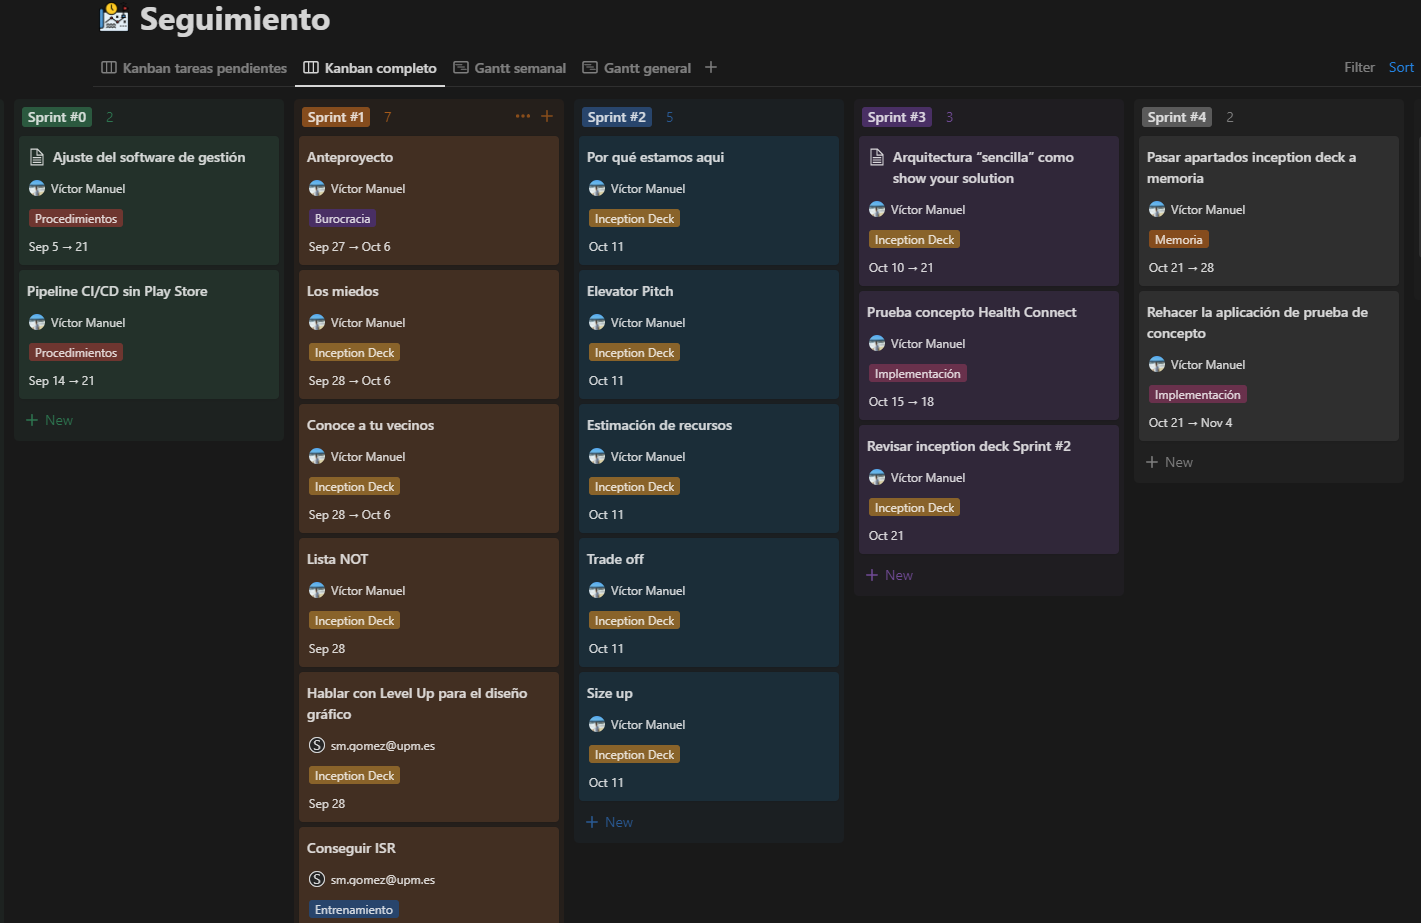
\includegraphics[width=0.75\textwidth]{figures/Kanban completo.PNG}
%            \caption{Extracto del tablero Kanban del proyecto}
%            \label{fig:notion:kanban}
%        \end{figure}
%    \item Diagrama Gantt. En esencia es una vista a la misma base de datos que la del tablero Kanban.
%        \begin{figure}[h!]
%            \centering
%            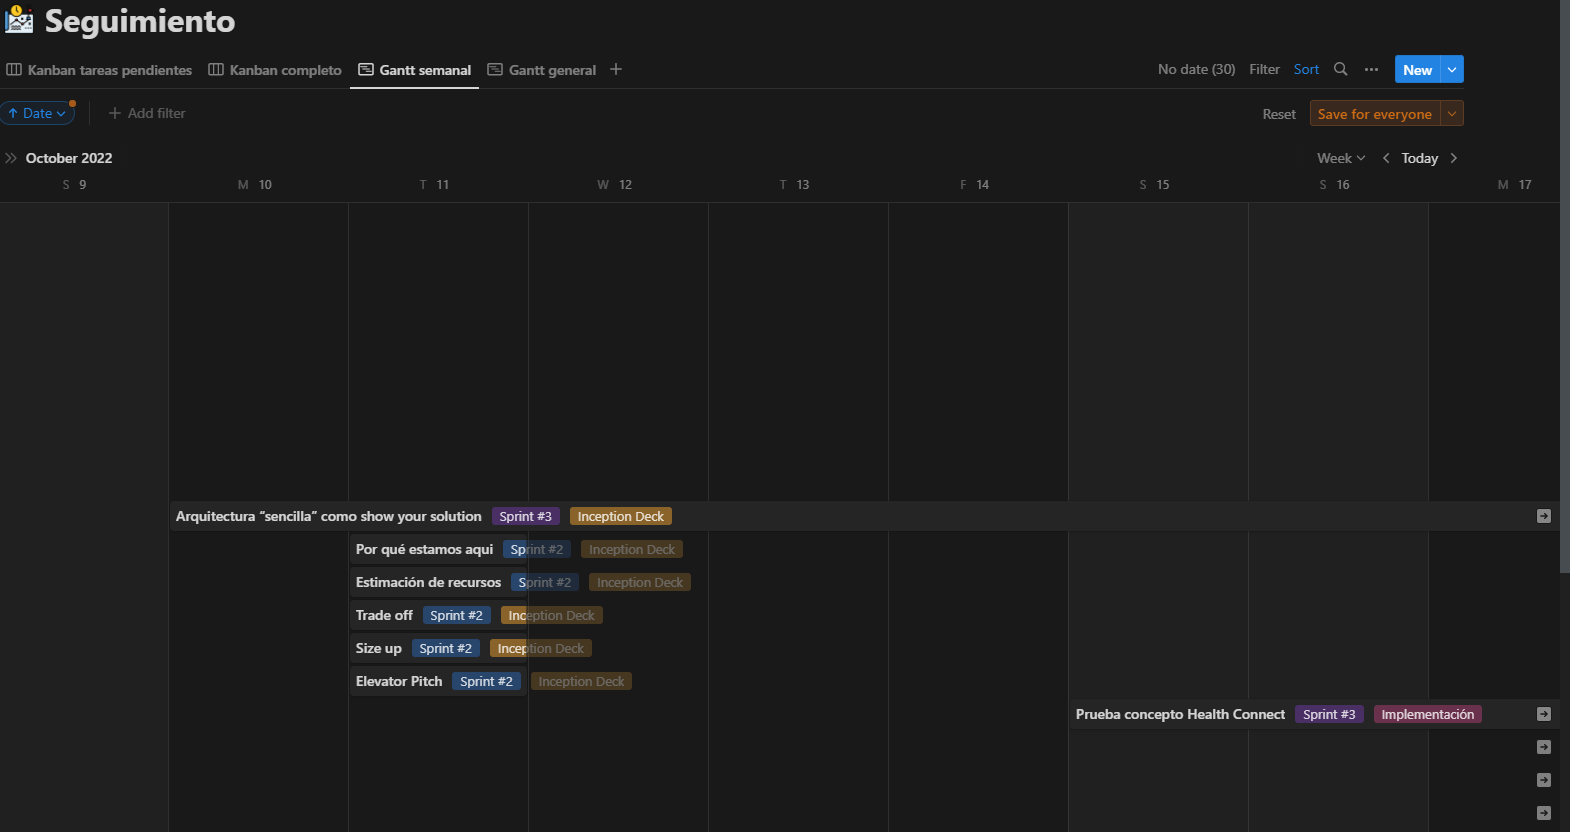
\includegraphics[width=0.75\textwidth]{figures/gantt semanal.PNG}
%            \caption{Extracto del diagrama Gantt del proyecto}
%            \label{fig:notion:gantt}
%        \end{figure}
%    \item Base de datos de referencias con todos los link de interés para la implementación del proyecto. Algunos de ellos aparecen en la bibliografía de esta memoria por su relevancia para exponer ciertas cuestiones.
%        \begin{figure}[h!]
%            \centering
%            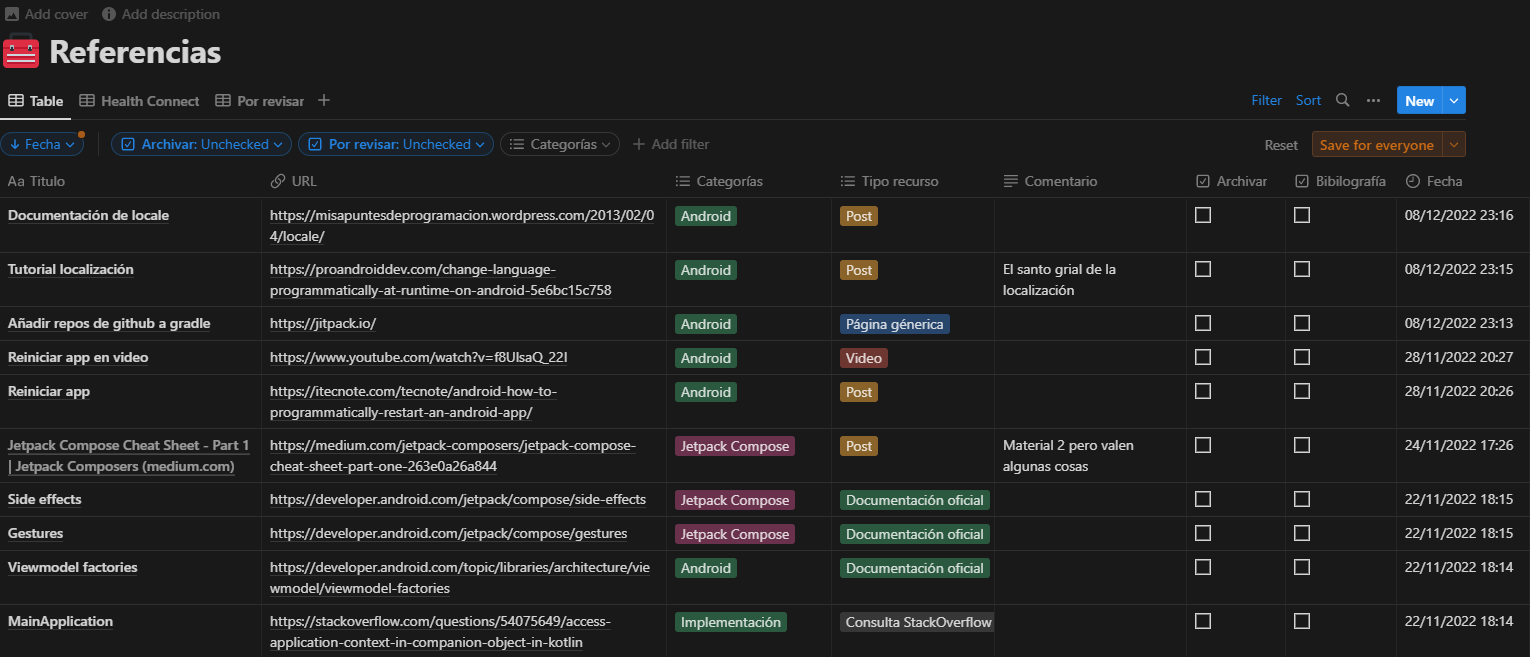
\includegraphics[width=0.75\textwidth]{figures/referencias.PNG}
%            \caption{Extracto de la base de datos de referencias}
%            \label{fig:notion:referencias}
%        \end{figure}
%    \item Base de datos con apuntes de consulta. Aquí se alojan descripciones de conceptos de utilidad para el proyecto. Está enlazada con la base de datos de referencia para acceder rápidamente a los enlaces para ampliar esa información.
%        \begin{figure}[h!]
%            \centering
%            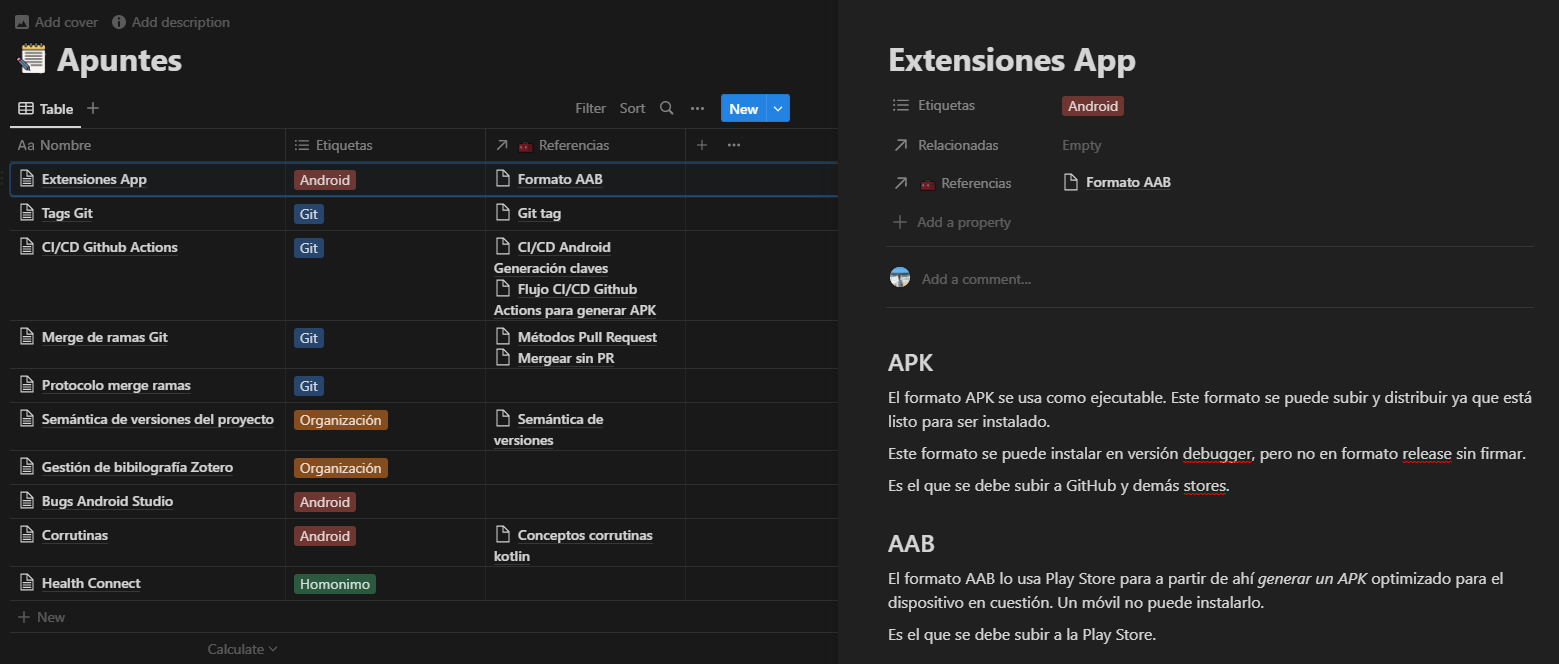
\includegraphics[width=0.75\textwidth]{figures/apuntes.PNG}
%            \caption{Extracto de la base de datos de apuntes del proyecto}
%            \label{fig:notion:apuntes}
%        \end{figure}
%\end{itemize}

\todo[inline]{hablar de los repositorios git y github}

\subsection*{Metodología del desarrollo seleccionada}

